\documentclass[a4paper,11pt]{scrartcl}

\usepackage{graphicx}
\usepackage[utf8]{inputenc} %-- pour utiliser des accents en français
\usepackage{amsmath,amssymb,amsthm} 
\usepackage[round]{natbib}
\usepackage{url}
\usepackage{xspace}
\usepackage[left=20mm,top=20mm]{geometry}
\usepackage{subcaption}
\usepackage{mathpazo}
\usepackage{booktabs}
\usepackage{hyperref}
\usepackage{graphicx}
% \usepackage{draftwatermark}
\graphicspath{{/media/maxence/SD_MAXENCE/cours/m1Informatique/S2/ATD/tp1_page_rank/ressource/}}
\newcommand{\ie}{ie}
\newcommand{\eg}{eg}
\newcommand{\reffig}[1]{Figure~\ref{#1}}
\newcommand{\refsec}[1]{Section~\ref{#1}}

\setcapindent{1em} %-- for captions of Figures


\title{TP K Moyenne}
\author{Grand Maxence}
\date{\today}


\begin{document}

\maketitle

\begin{center}
  \textbf{Sixi\`eme ex\'ecution}\par\medskip
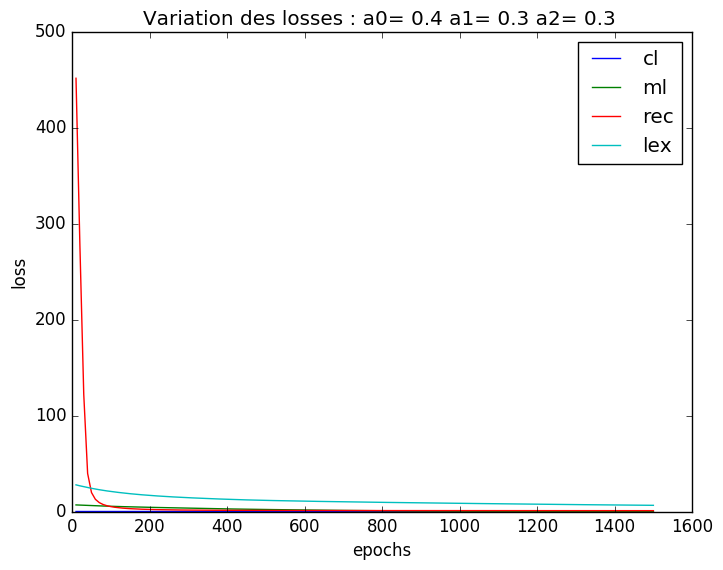
\includegraphics[width=0.6\textwidth]{test6.png}
\end{center}
\begin{center}
  \textbf{Dixi\`eme ex\'ecution}\par\medskip
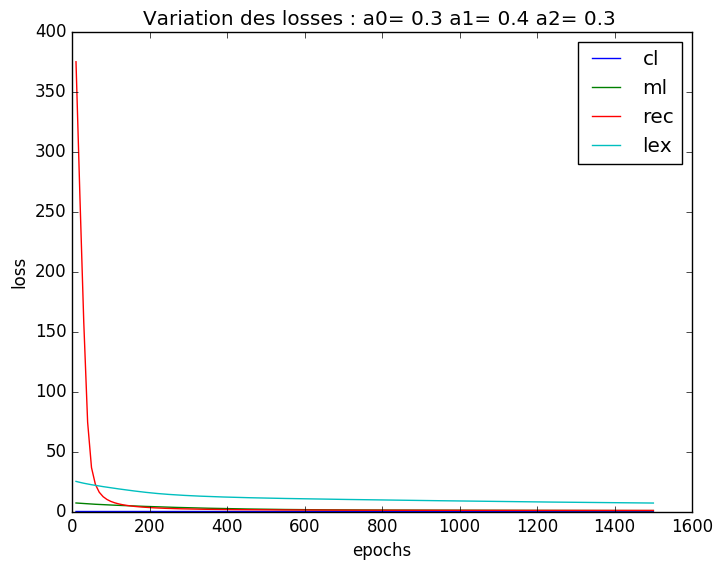
\includegraphics[width=0.6\textwidth]{test10.png}
\end{center}
Nous observons que les deux r\'esultats ci-dessus sont diff\'erents. Cela vient
de l'initiaisation des centroids. En effet il est possible que les centroids
initiaux pousse vers une solution locale. Pour \'eviter de tomber dans une solution
locale, il faudrait que les centroids soient initialis\'es le plus proche possible des
centroids de la solution globale.

\begin{center}
\includegraphics[width=1\textwidth]{nmi.png}
\end{center}

Nous observons que la NMI est \`a peu pr\`es stable, except\'e pour la dixi\`eme
ex\'ecution.

\end{document}
